\section{GUI}
The GUI starts by running command \texttt{python3 main.py} in the virtual environment.

\subsection{Login screen}
When the app is opened, the user is greeted by a login screen. The user can either log in with an existing account if they used the app in the past as shown in Figure \ref{fig:login} or create a new one with username and password as in Figure \ref{fig:reg}.
\begin{figure}[h]
    \centering
    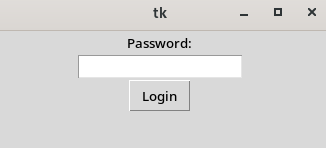
\includegraphics[width=0.5\textwidth]{images/login.png}
    \caption{Login screen}
    \label{fig:login}
\end{figure}

\begin{figure}[h]
    \centering
    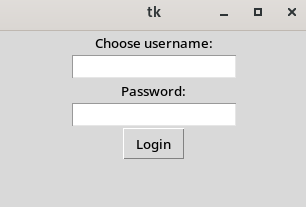
\includegraphics[width=0.5\textwidth]{images/register.png}
    \caption{Register screen}
    \label{fig:reg}
\end{figure}

\newpage

\subsection{Main window}
After the login, the user will see the main application window. 
\begin{figure}[h]
    \centering
    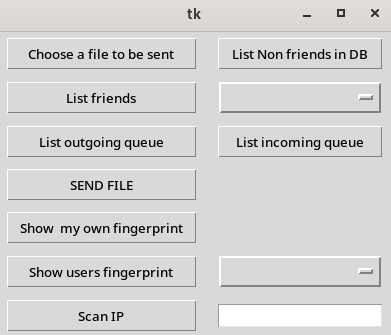
\includegraphics[width=0.5\textwidth]{images/mainwindow.png}
    \caption{Main window}
    \label{fig:main}
\end{figure}

\subsubsection{File selection}
Selecting a file for transfer is done by using the button \texttt{Choose a file to be sent} that is shown in Figure \ref{fig:main}. 
After pressing the button, the file selection window will open and user can select the file they want to send.

\subsubsection{User discovery and friend addition}
There are 2 ways to discover other users who are using the app. Either the user can scan the whole network for active apps that are running using \texttt{List Non friends in DB} button.
\begin{figure}[h]
    \centering
    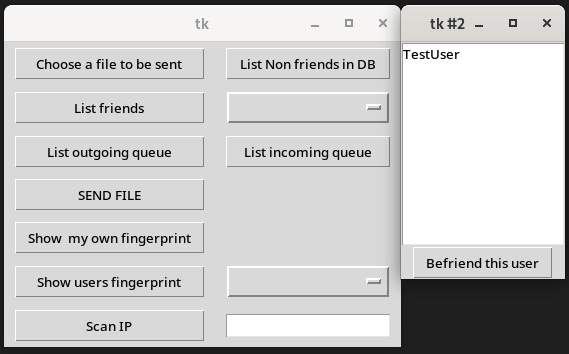
\includegraphics[width=0.5\textwidth]{images/ListNonFriends.png}
    \caption{Adding users to db by scanning the network}
    \label{fig:LNF}
\end{figure}

The other way is by using button \texttt{Scan IP}. User enters the address they want to scan in the text field next to the button and then presses the button.
\begin{figure}[h]
    \centering
    
\includegraphics[width=0.5\textwidth]{images/ScanIP.png}
    \caption{Adding user to db by scanning given IP}
    \label{fig:scanIP}
\end{figure}

Adding friends is handled by pressing the button \texttt{Befriend this user} that we can see in Figure \ref{fig:LNF}.

\subsubsection{Listing of users}
There are 2 ways to list other users that the user can interact with. Either list only those users who the user added to their friend list or list all users in database.
For this there are 2 buttons shown on Figure \ref{fig:main}. Those are \texttt{List friends} and \texttt{List Non friends in DB} respectively.

\subsubsection{Listing queued files}
Files that cannot be sent immediately are queued and will be sent once the user is available. The user can see the list of queued files by pressing the button 
\texttt{List outgoing queue}.\\

\subsubsection{Friend selection}
Choosing a friend who will be the target of the file transfer is done by choosing one friend from the drop-down menu next to the \texttt{List friends} button.\\

\subsubsection{Fingerprints}
There are 2 buttons regarding the fingerprints. The first one is \texttt{Show my own fingerprint} so the user can look up their certificate fingerprint. The \texttt{Show users fingerprint} button is paired with a drop-down menu, where the user can choose whose fingerprint they want to see in case they want to verify that the fingerprint is correct and they are not falling victim for some kind of MitM attack.\\
\subsubsection{File sharing}
After selecting the file and the friend to send it to, the user can press the button \texttt{Send file} to send the file to the selected friend.
If the target is not available, the app will prompt the user with following message and put the file in the queue to be sent later.
\begin{figure}[h]
    \centering
    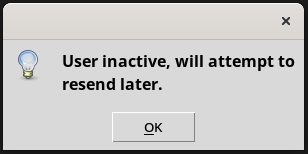
\includegraphics[width=0.5\textwidth]{images/notAvailable.png}
    \caption{Target not available}
    \label{fig:notAvail}
\end{figure}

Receiving the file is done by the target user pressing the button \texttt{List incoming queue} which opens window with all files that are waiting to be
received. The user can either save or ignore a single file or accept all files in the queue.\\

\begin{figure}[ht]
    \centering
    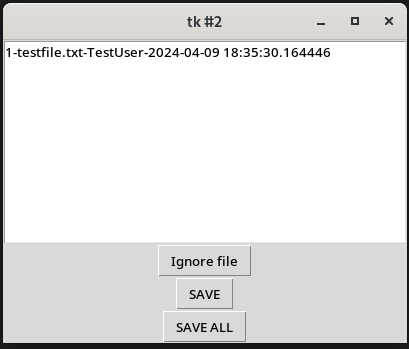
\includegraphics[width=0.5\textwidth]{images/queue.png}
    \caption{Incoming queue}
    \label{fig:inQueue}
\end{figure}

If the user chooses to save the file they are prompted with a window to select the location where the file will be saved.\\